\documentclass[tikz]{standalone}
\usepackage{pgfplots}
\usepgfplotslibrary{groupplots}
\pgfplotsset{compat=1.18}
\definecolor{utnblue}{RGB}{0, 102, 204}

\begin{document}
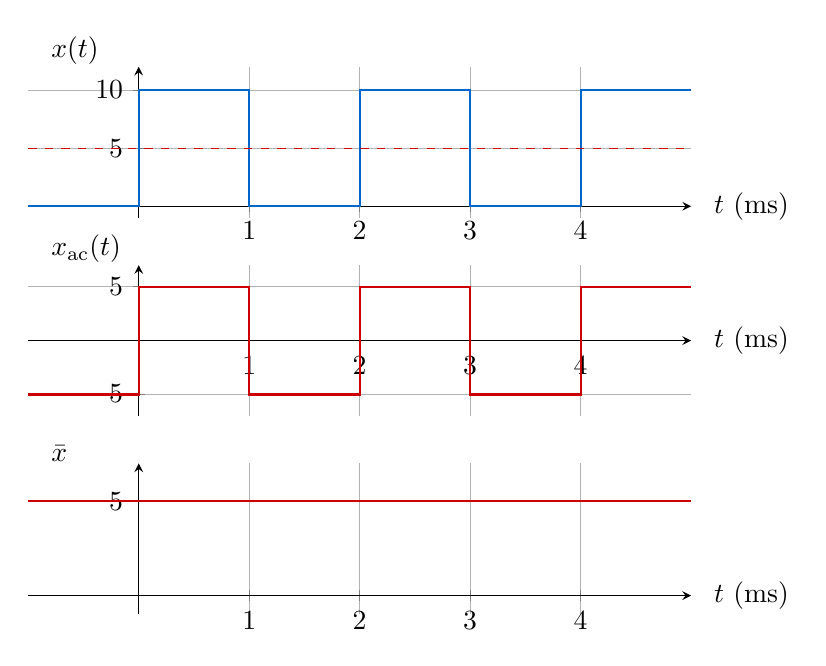
\begin{tikzpicture}
    \begin{groupplot}[
        group style={
            group size=1 by 3,
            vertical sep=0.6cm,
        },
        width=10cm,
        height=3.5cm,
        axis lines=middle,
        grid=both,
        grid style={line width=.1pt, draw=gray!40},
        major grid style={line width=.2pt,draw=gray!60},
        every axis plot/.append style={thick},
        every axis x label/.append style={at={(ticklabel* cs:1.02)}, anchor=west},
        every axis y label/.append style={at={(rel axis cs:0.02, 0.95)}, anchor=south west, rotate=0},
    ]
    
    % Panel 1: x(t) señal cuadrada original
    \nextgroupplot[
        xmin=-1, xmax=5, ymin=-1, ymax=12,
        xtick={0,1,2,3,4}, ytick={0,5,10},
        ylabel={$x(t)$}, xlabel={$t$ (ms)},
    ]
    \addplot[utnblue] coordinates {(-1,0) (0,0) (0,10) (1,10) (1,0) (2,0) (2,10) (3,10) (3,0) (4,0) (4,10) (5,10)};
    \draw[dashed, red!80!black] (axis cs:-1,5) -- (axis cs:5,5) node[right, font=\footnotesize] {$\bar{x}=5$};
    
    % Panel 2: x_ac(t) componente alterna
    \nextgroupplot[
        xmin=-1, xmax=5, ymin=-7, ymax=7,
        xtick={0,1,2,3,4}, ytick={-5,0,5},
        ylabel={$x_\mathrm{ac}(t)$}, xlabel={$t$ (ms)},
    ]
    \addplot[red!80!black] coordinates {(-1,-5) (0,-5) (0,5) (1,5) (1,-5) (2,-5) (2,5) (3,5) (3,-5) (4,-5) (4,5) (5,5)};
    
    % Panel 3: DC constante
    \nextgroupplot[
        xmin=-1, xmax=5, ymin=-1, ymax=7,
        xtick={0,1,2,3,4}, ytick={0,5},
        ylabel={$\bar{x}$}, xlabel={$t$ (ms)},
    ]
    \addplot[red!80!black] coordinates {(-1,5) (5,5)};
    
    \end{groupplot}
\end{tikzpicture}
\end{document}
